\documentclass[11pt,a4paper]{article}
\usepackage[margin=25mm]{geometry}
\usepackage[T1]{fontenc}
\usepackage[utf8]{inputenc}
\usepackage{lmodern,microtype,graphicx,booktabs,longtable,array,amsmath,amssymb,caption,placeins}
\usepackage[numbers,sort&compress]{natbib}
\usepackage[hidelinks]{hyperref}
\graphicspath{{figures/main/}}
\captionsetup{font=small,labelfont=bf}
\setlength{\emergencystretch}{2em}
\newcommand{\ExtensionModel}{random forest}
\newcommand{\ExtensionFOne}{0.821}
\newcommand{\ExtensionCV}{0.695}
\newcommand{\ExtensionLow}{0.691}
\newcommand{\ExtensionHigh}{0.835}
\newcommand{\ExtensionAgreement}{0.813}

\title{Sensitivity-aware inspection prioritisation for archaeological landscapes: a reproducible Taxila observatory}
\author{}
\date{}
\begin{document}
\maketitle
\begin{abstract}
Distributed archaeological landscapes require spatially explicit monitoring because limited field capacity must be directed among components exposed to different combinations of land-surface change, terrain, drainage and climate forcing. This problem is acute at the Taxila World Heritage property in Pakistan, where multiple archaeological components occur within a heterogeneous peri-urban landscape. Existing geospatial assessments rarely combine comparable multi-temporal observations with acquisition-window weather, scale sensitivity, indicator redundancy and uncertainty in the resulting inspection order. This study developed the Climate-linked Heritage Inspection Prioritisation (CHIP) framework to integrate those evidence streams while preserving the distinction between landscape pressure and verified heritage condition. The analysis used 55 Landsat scenes organised into five post-monsoon epochs from 2003--2005 to 2023--2025, daily gridded weather for 1991--2025, approximately 30~m elevation data, and WorldCover-derived proxy land-cover labels. Seventeen of 18 inventoried components had usable geometry. Satellite indicators were compared on common support, climate trends and antecedent acquisition windows were characterised, terrain and drainage features were aggregated at 250, 500 and 1,000~m, and a hierarchical relative-priority score was tested through ablation, 50,000 weight perturbations and 2,000 spatial-block resamples. Common endpoint support comprised 386,280 cells, or 95.7371\% of the fixed grid; 16.9284\% met at least two adverse spectral criteria and 1.4220\% met all three. At the primary 500~m support, the Giri complex had the highest fixed score, 0.591176, but its central 95\% rank interval under weight perturbation extended from 1 to 9. Spatial resampling instead gave Bhallar median rank 1 and Giri median rank 2, with overlapping intervals. The 500 and 1,000~m rankings agreed more closely (Spearman $\rho=0.91846$) than the 250 and 1,000~m rankings ($\rho=0.71078$). A geographically buffered proxy experiment achieved a macro-averaged F1 score of 0.830795 on 4,188 held-out samples, but measured agreement with proxy land-cover labels only. CHIP therefore supports tiered field-inspection sequencing and mechanism-specific survey questions rather than an unqualified single-site ranking. It does not demonstrate monument damage, deterioration probability or a legally defined risk zone.
\end{abstract}
\noindent\textbf{Keywords:} cultural heritage; archaeological landscapes; Earth observation; multi-temporal Landsat; climate variability; terrain hydrology; spatial uncertainty; sensitivity analysis; field-inspection prioritisation; Taxila.

\section{Introduction}
Archaeological conservation requires decisions across spatial scales: monument fabric, its immediate surroundings and the wider landscape. Satellite observations, terrain models and weather products capture different parts of this system. Translating them into an inspection programme requires more than overlaying indicators: the resulting priorities must be traceable to their environmental drivers and stable enough for a defined management task.

Remote sensing and GIS have documented development pressure and supported heritage multi-hazard assessment \citep{agapiou2015paphos,agapiou2016paphos,guerriero2022derwent}. At Taxila, Khan et al. integrated ground-based and satellite evidence for hazard assessment \citep{khan2022taxila}; Butt et al. subsequently examined land-cover transitions and urban encroachment over 1990--2024 \citep{butt2025taxila}. These studies establish the local conservation problem. Recent work by Megarry et al. extends the relevance of surrounding land cover to climate-vulnerability assessment across cultural World Heritage properties in the Indian Subcontinent \citep{megarry2026landcover}. The next decision-oriented question is whether an inspection set persists when spatial support, indicator composition and decision weights change. Mapping pressure and evaluating the stability of a management recommendation are complementary contributions.

GIS multicriteria methods formalise indicator aggregation, while sensitivity analysis reveals dependence on weights and spatial representation \citep{malczewski2006gis,feizizadeh2014uncertainty}. Rank-acceptability methods further describe which alternatives remain preferred under uncertain criteria and preferences \citep{lahdelma2001smaa}. For archaeological landscapes, these ideas motivate an experimental treatment of priority construction: correlated proxies can duplicate information, neighbouring buffers can share observations, and uncertain coordinates can alter the sampled environment. A single final ranking leaves these dependencies unresolved.

Climate interpretation introduces temporal-support constraints. Exposure depends on materials, maintenance, drainage and microenvironment alongside meteorological forcing \citep{sesana2021climate,sesana2020vulnerability,crowley2022risk}. Acquisition-matched weather and cross-product comparison can test whether a proposed explanation is consistent with the observations. Separately, predictive evaluation must distinguish geographic land-cover transfer from conservation-condition assessment. Spatially nearby samples can share predictors and labels \citep{hijmans2012cv,roberts2017cv,meyer2021aoa}; reproducing a global land-cover product does not establish monument deterioration.

We develop CHIP as an experimentally evaluated inspection framework with three contributions. First, a hierarchical landscape--terrain rule exposes indicator influence through baselines and ablations, and exact weight crossings identify where inspection leadership changes. Second, multiscale, shared-block, positional and nested spatial--decision experiments distinguish persistent priorities from representation-dependent ones. Third, acquisition-matched climate comparisons and a seven-family buffered land-cover benchmark evaluate the environmental and predictive evidence supporting interpretation. The resulting inspection portfolio retains both a persistent component set and the mechanisms that require field verification.

\section{Research aim}
The study identifies which Taxila components merit early field inspection and which parts of that recommendation depend on analytical choices. It tests adverse spectral convergence on common spatial support, changes in climate interpretation across acquisition windows and products, rank stability across neighbourhoods and uncertainty designs, and land-cover proxy agreement under buffered spatial evaluation. Mathematical definitions connect these experiments to reproducible component-level decisions.

\section{Materials and methods}
\subsection{Study area, inventory and evidence sources}
Taxila is a serial World Heritage property in Punjab, Pakistan, inscribed under reference 139 \citep{unesco_taxila}. The inventory contained 18 component records. Seventeen had usable point coordinates; Saraikala (139-002) remained in the documentary inventory but was excluded from coordinate-dependent analysis because its location was unresolved. Spectral neighbourhoods used WGS 84/UTM zone 43N (EPSG:32643); terrain extraction used local metric approximations on the geographic elevation grid. Point-centred circles of 250, 500 and 1,000 m defined analytical neighbourhoods, with 500 m used for primary reporting. They are neither official property polygons nor statutory or UNESCO buffer zones (Fig.~\ref{fig:study}).

\begin{figure}[tbp]\centering
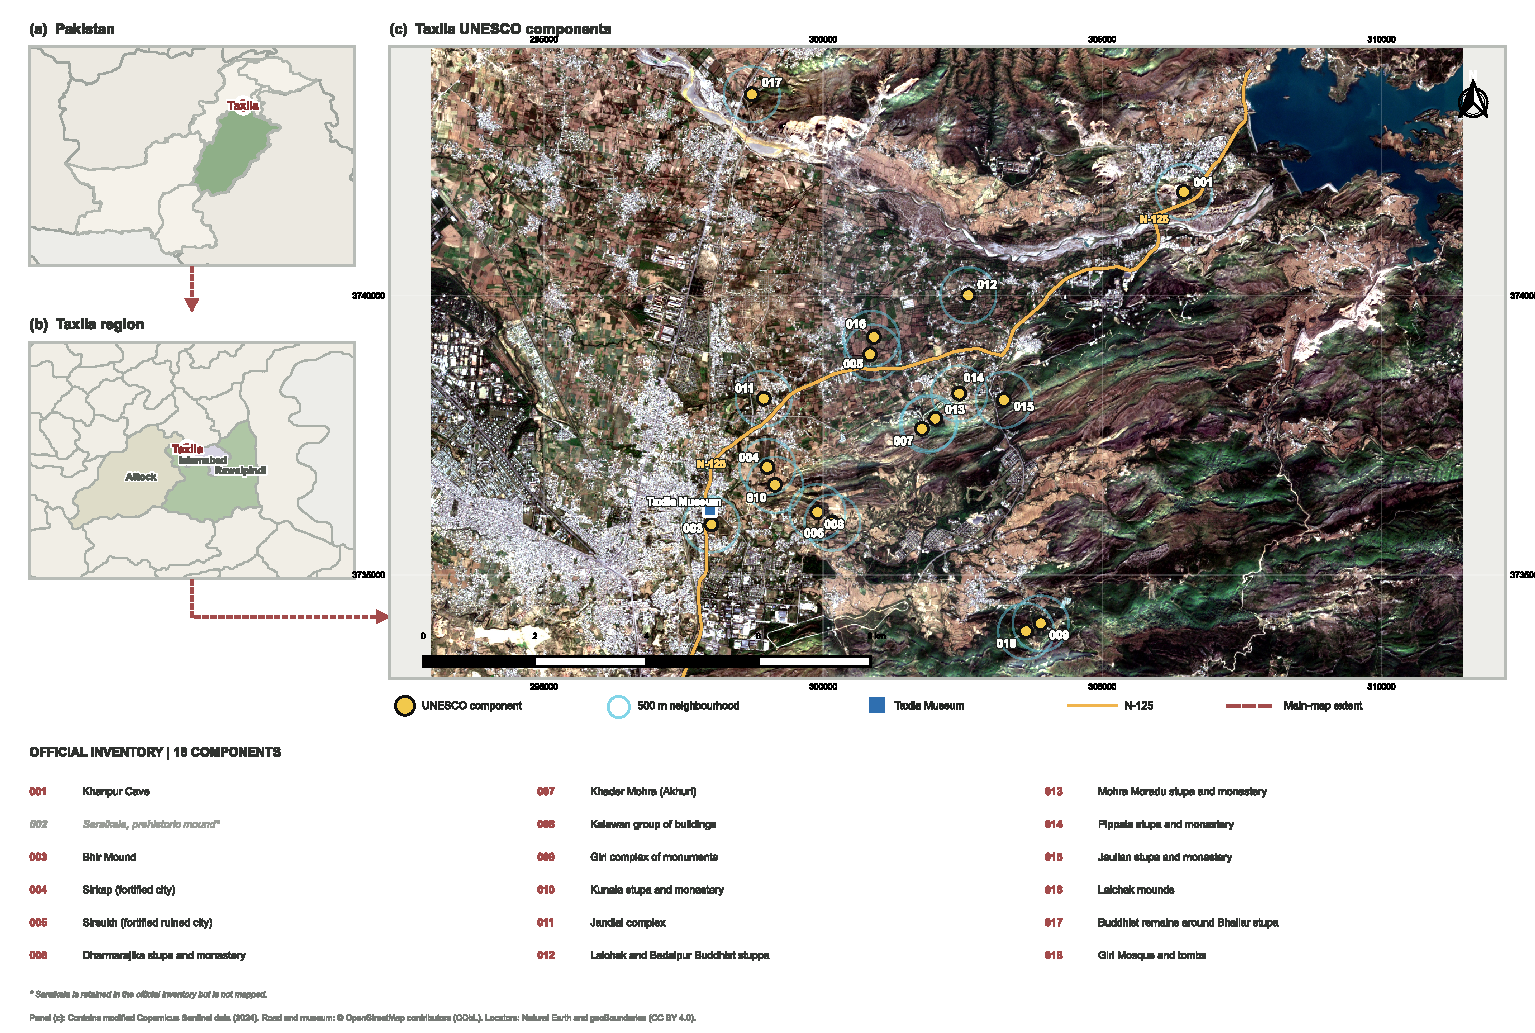
\includegraphics[width=\textwidth]{figure_01_study_area_context_map.pdf}
\caption{Taxila study-area context and the official 18-component inventory. Seventeen components are mapped; Saraikala is retained in the inventory without an inferred coordinate. Dark-red circles indicate 500 m analytical neighbourhoods. Esri World Imagery provides contextual imagery only; it was not used to calculate spectral, climate or terrain indicators. Boundaries: Natural Earth and geoBoundaries; road and museum: OpenStreetMap contributors (ODbL). Map lines delineate study areas and do not necessarily depict accepted national boundaries. }\label{fig:study}
\end{figure}

Landsat Collection 2 Level-2 surface reflectance supplied five post-monsoon three-year composites: 2003--2005, 2008--2010, 2013--2015, 2018--2020 and 2023--2025, abbreviated E2004 to E2024. They contained 11, 10, 8, 8 and 18 retained scenes, respectively. Landsat 7 supplied the first two epochs, Landsat 8 the middle two, and Landsat 8/9 the final epoch. Source records preserve acquisition dates, sensor identities and quality information. Cross-sensor and masking limitations were considered explicitly \citep{usgs_landsat_c2,roy2016landsat}.

Daily Open-Meteo ERA5-Seamless data covered 1991--2025 \citep{openmeteo_archive}. Component queries resolved to four unique weather cells, each containing 12,784 daily records. NASA POWER supplied a comparison product over the same period \citep{nasa_power}. Neither was treated as station truth. Terrain came from the one-arc-second N33E072 elevation tile distributed through AWS Terrain Tiles. ESA WorldCover 2020/2021 consensus \citep{esa_worldcover} supplied six proxy land-cover classes for an E2019 feature table. Table~\ref{tab:data} summarises the role of each source. Figure~\ref{fig:framework} separates the paths through which these inputs inform interpretation.

\begin{table}[tbp]\centering\small
\caption{Evidence sources and permitted analytical roles.}\label{tab:data}
\begin{tabular}{p{.22\linewidth}p{.30\linewidth}p{.38\linewidth}}\toprule
Source & Support & Analytical role \\\midrule
Landsat C2 L2 & 55 scenes; five epochs; 30 m grid & Relative spectral pressure and endpoint convergence \\
Elevation tile & Approximately 30 m & Terrain and drainage susceptibility \\
Open-Meteo & Daily, 1991--2025; four cells & Regional trends and acquisition-window context \\
NASA POWER & Daily, 1991--2025 & Weather-product sensitivity \\
WorldCover consensus & 2020/2021 labels matched to E2019 features & Weakly supervised land-cover benchmark \\
UNESCO component inventory & 18 records; 17 mapped points & Component identifiers and neighbourhood centres \\\bottomrule
\end{tabular}
\end{table}

\begin{figure}[p]\centering
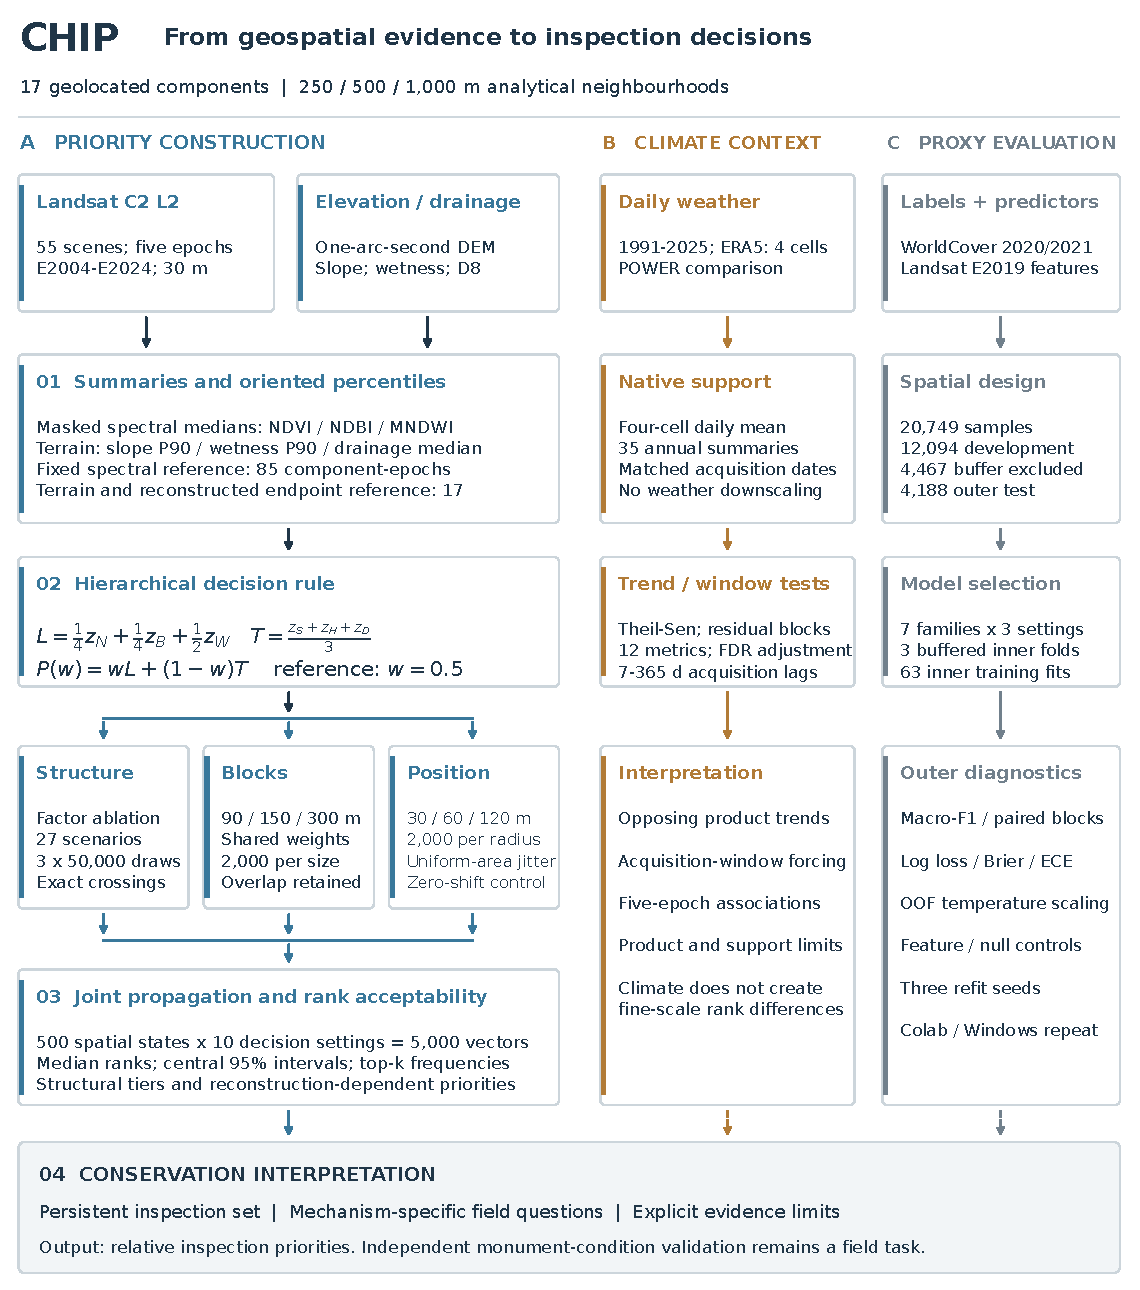
\includegraphics[width=\textwidth]{figure_02_chip_framework.pdf}
\caption{CHIP framework linking observation support, mathematical transformations, experiments and conservation interpretation. Solid arrows carry analytical inputs; dashed arrows carry interpretation. Climate retains native support and land-cover evaluation remains a separate diagnostic. Fixed and reconstructed spectral percentile populations are distinguished. Counts describe executed designs. Codex assisted this editable vector schematic.}\label{fig:framework}
\end{figure}


\subsection{Spectral transformations and common-support convergence}
Cloud, shadow and invalid observations were masked before compositing on a fixed 30 m grid. With scaled reflectance $\rho_b$ in band $b$, the indices were
\begin{equation}\label{eq:indices}
\mathrm{NDVI}=\frac{\rho_{\mathrm{NIR}}-\rho_{\mathrm{red}}}{\rho_{\mathrm{NIR}}+\rho_{\mathrm{red}}},\quad
\mathrm{NDBI}=\frac{\rho_{\mathrm{SWIR1}}-\rho_{\mathrm{NIR}}}{\rho_{\mathrm{SWIR1}}+\rho_{\mathrm{NIR}}},\quad
\mathrm{MNDWI}=\frac{\rho_{\mathrm{green}}-\rho_{\mathrm{SWIR1}}}{\rho_{\mathrm{green}}+\rho_{\mathrm{SWIR1}}}.
\end{equation}
These ratios follow their original definitions \citep{tucker1979ndvi,zha2003ndbi,xu2006mndwi}. NDBI responds to bare soil as well as built surfaces; its adverse direction is a screening assumption, not an attribution of urban expansion.

For component $i$, epoch $e$, radius $r$ and factor $k$, let $x_{ierk}$ denote the neighbourhood median. The oriented empirical percentile is
\begin{equation}\label{eq:percentile}
z_{ierk}=\frac{\operatorname{rank}_{\mathcal I_r}(s_kx_{ierk})-\tfrac12}{N_r},
\qquad s_N=s_W=-1,\quad s_B=+1.
\end{equation}
Ranks ascend with average ties; $N_r=|\mathcal I_r|=85$ component--epoch observations at each radius ($17\times5$). Terrain percentiles use the 17 static component summaries. Spatial reconstruction experiments instead rerank the 17 simultaneously reconstructed E2024 summaries. Reconstruction differences therefore include a reference-population effect. Percentiles describe relative evidence within their stated population, not transferable physical thresholds.

Endpoint differences $\Delta I_k(p)=I_{k,\mathrm{E2024}}(p)-I_{k,\mathrm{E2004}}(p)$ used only the common valid-cell set $\Omega$. With $Q_k(q)$ denoting its empirical $q$-quantile,
\begin{equation}\label{eq:convergence}
\begin{aligned}
C(p)&=\mathbf1[\Delta I_N(p)\leq Q_N(.2)]+\mathbf1[\Delta I_W(p)\leq Q_W(.2)]
       +\mathbf1[\Delta I_B(p)\geq Q_B(.8)],\\
\pi_{\geq h}&=|\Omega|^{-1}\sum_{p\in\Omega}\mathbf1[C(p)\geq h],\qquad h\in\{2,3\}.
\end{aligned}
\end{equation}
The indicator function $\mathbf1[\cdot]$ equals one when its condition holds. These overlapping, data-derived tails quantify descriptive convergence; they are neither independent tests nor measurements of damaged area.

\subsection{Terrain representation and hierarchical decision rule}
D8 routing directs each elevation cell to its steepest strictly lower neighbour; sinks remain terminal. Slope $\theta$ derives from metric elevation gradients. The contributing-cell count $A_c$ and geometric-mean cell width $h$ define the numerical wetness proxy
\begin{equation}\label{eq:wetness}
H(p)=\log\!\left[\frac{(A_c(p)+1)\,h/(1\,\mathrm{m})}
 {\tan(\max\{\theta(p),0.05^\circ\})+0.01}\right].
\end{equation}
This regularised topographic proxy follows the contributing-area/slope rationale of hydrological terrain analysis \citep{beven1979topmodel,moore1991terrain}. Drainage comprises cells at or above the 99th percentile of accumulation. Component factors are the 90th percentiles of slope and $H$, and median Euclidean drainage distance. Higher slope and wetness and shorter distance are oriented towards greater susceptibility. Routing approximates topographic convergence, not discharge, and omits unresolved walls, culverts and local drains.

With $S,H,D$ indexing slope, wetness and drainage proximity, landscape pressure $L$, terrain susceptibility $T$ and priority $P$ are
\begin{equation}\label{eq:priority}
\begin{aligned}
L_{ier}&=\tfrac14z_{ierN}+\tfrac14z_{ierB}+\tfrac12z_{ierW},\\
T_{ir}&=\tfrac13(z_{irS}+z_{irH}+z_{irD}),\\
P_{ier}(w)&=wL_{ier}+(1-w)T_{ir},\qquad P_{ier}^{\mathrm{ref}}=P_{ier}(0.5).
\end{aligned}
\end{equation}
Grouping NDVI and NDBI limits their combined weight relative to MNDWI without claiming statistical independence. Equal domain weights are declared choices, not fitted conservation parameters. This hierarchical construction connects GIS multicriteria assessment \citep{malczewski2006gis} to explicitly testable sensitivity assumptions \citep{chen2010sensitivity,feizizadeh2014uncertainty}. A regional climate term remains contextual: adding the same value to every component through an equal-weight integrated score is an affine transformation of $P^{\mathrm{ref}}$ and cannot alter the within-epoch ordering.

\subsection{Structural experiments and exact weight transitions}
The hierarchy was compared with an equal six-factor mean, landscape-only and terrain-only baselines. Factor ablations removed one term and renormalised retained weights. Spearman correlation, Kendall concordance, top-five overlap and maximum rank displacement describe ordering changes.

Three radii, three landscape weights ($0.25,0.50,0.75$) and three terrain formulations produce 27 scenarios. Terrain alternatives comprise equal factors, inverse-correlation weights and the reduced slope--drainage mean. For the correlation-adjusted case, $a_k\propto[\sum_\ell|\rho_{k\ell}|]^{-1}$ with $\sum_ka_k=1$, where $\rho$ is the Spearman matrix of the three terrain factors, including its diagonal. Continuous-weight experiments sample $w\sim\mathrm{Beta}(\alpha,\alpha)$ for $\alpha\in\{0.5,1,2\}$, with 50,000 draws each. This evaluates stated preference distributions rather than inferring stakeholders' preferences, consistent with rank-acceptability analysis \citep{lahdelma2001smaa}.

An additional deterministic analysis resolves every pairwise score crossing. For E2024 components $i,j$ at fixed radius and equal-factor terrain, solving $P_i(w)=P_j(w)$ gives
\begin{equation}\label{eq:crossing}
w^*_{ij}=\frac{T_j-T_i}{(L_i-T_i)-(L_j-T_j)}.
\end{equation}
Only nonzero denominators and crossings in $(0,1)$ are retained. Sorting these crossings partitions the weight interval into regions of constant rank order; midpoint evaluation identifies the leader in each region. Boundary ties retain component-inventory order. Figure~\ref{fig:scales} combines fixed ranks, a three-dimensional rank response and exact leadership intervals. Radii remain discrete; no interpolated spatial-resolution surface is implied.

\subsection{Spatial, positional and joint uncertainty propagation}
At each block size (90, 150, 300 m), 2,000 spatial draws used shared exponential weights. If $m_{ibk}$ is the median of factor $k$ in block $b$ intersecting component $i$, and $n_{ib}$ its valid-cell count,
\begin{equation}\label{eq:block}
E_b^{(d)}\sim\operatorname{Exp}(1),\quad v_{ib}^{(d)}=n_{ib}E_b^{(d)},\quad
\widetilde x_{ik}^{(d)}=\operatorname{wmed}_{b}\{m_{ibk};v_{ib}^{(d)}\}.
\end{equation}
The weighted median is the first ordered block median reaching half the cumulative weight. Sharing $E_b^{(d)}$ across overlapping neighbourhoods preserves their resampling dependence; cell counts retain unequal spatial support. Terrain remains fixed in this experiment.

For positional sensitivity, independent uniform-area displacements are
\begin{equation}\label{eq:displacement}
\boldsymbol\delta_i=d_{\max}\sqrt{U_i}(\cos\phi_i,\sin\phi_i),\quad
U_i\sim U(0,1),\quad \phi_i\sim U(0,2\pi).
\end{equation}
Spectral and terrain summaries were re-extracted for 2,000 draws at each $d_{\max}\in\{30,60,120\}$ m. An undisplaced re-extraction supplies the appropriate control. Equation~\eqref{eq:percentile} distinguishes this endpoint reference from the fixed summary-table reference.

Joint simulation generates 500 spatial states, each with sampled block size, shared block weights and independent displacement within 120 m. Ten decision settings per state sample $w\sim U(0,1)$ and one terrain formulation. For resulting ordinal ranks $R_i^{sd}$, top-$k$ frequency is
\begin{equation}\label{eq:acceptability}
\widehat b_i(k)=\frac{1}{500\times10}\sum_{s=1}^{500}\sum_{d=1}^{10}
 \mathbf1[R_i^{sd}\leq k].
\end{equation}
Median ranks and central 95\% intervals summarise these 5,000 nested score vectors. They are conditional sensitivity distributions, not 5,000 independent maps or posterior probabilities of deterioration. The same frequency definition over 27 structural scenarios defines a core tier at $b_i(3)\geq0.5$ and a conditional tier outside it at $b_i(5)\geq0.5$.

\subsection{Climate trends and acquisition-matched forcing}
The regional daily series averages four unique weather cells equally before annual aggregation. For annual values $Y_t$, the Theil--Sen estimator is
\begin{equation}\label{eq:sen}
\widehat\beta=\operatorname{median}_{u>t}\frac{Y_u-Y_t}{u-t}.
\end{equation}
After robust trend fitting, five-year residual blocks were resampled and the fitted trend restored to obtain 2,000 slope replicates \citep{sen1968slope,yue2002autocorrelation}. Null replicates add resampled residuals to a constant baseline. The two-sided probability is $(1+\sum_b\mathbf1[|\beta_b^0|\geq|\widehat\beta|])/(2,001)$; Benjamini--Hochberg adjustment covers 12 annual metrics \citep{benjamini1995fdr}. Inference assumes adequate representation of short-range residual dependence and remains conditional on the weather product.

For acquisition dates $a\in\mathcal A_e$, daily precipitation $W(t)$ and antecedent window $\ell$,
\begin{equation}\label{eq:lags}
\overline W_e(\ell)=\frac{1}{|\mathcal A_e|}\sum_{a\in\mathcal A_e}
 \sum_{u=1}^{\ell}W(a-u),\qquad \ell\in\{7,30,90,180,365\}\ \mathrm{days}.
\end{equation}
Temperature uses window means. Product comparisons match dates and periods. Five composite epochs provide only five temporal replicates for exploratory weather--spectral associations; no weather field was downscaled to 30 m.

\subsection{Buffered model selection and probability diagnostics}
The weakly supervised benchmark contained 20,749 class-stratified samples, six reflectance bands and four indices. Its outer stripe contained 4,188 samples in 20 blocks; 4,467 samples in adjacent block columns were excluded, leaving 12,094 development samples in 60 blocks. Three contiguous inner validation bands each excluded an adjacent block row from training. This design targets geographical transfer \citep{roberts2017cv,meyer2018target}, with class-stratified agreement interpreted separately from population-area map accuracy \citep{olofsson2014accuracy,stehman2019accuracy}.

Seven families---logistic regression, random forest, extra trees, histogram gradient boosting, MLP, XGBoost and CatBoost---each received three predeclared configurations \citep{breiman2001rf,pedregosa2011sklearn,chen2016xgboost,prokhorenkova2018catboost}. The resulting 63 inner fits selected family $m$ and configuration $\eta$ through
\begin{equation}\label{eq:selection}
\begin{aligned}
(\widehat m,\widehat\eta)&=\arg\max_{m,\eta}\frac13\sum_{v=1}^{3}
 F_{1,\mathrm{macro}}(y_v,\widehat f_{m,\eta}^{(-v)}(X_v)),\\
F_{1,\mathrm{macro}}&=\frac16\sum_{c=1}^{6}
 \frac{2\mathrm{TP}_c}{2\mathrm{TP}_c+\mathrm{FP}_c+\mathrm{FN}_c}.
\end{aligned}
\end{equation}
Undefined class terms receive zero. Water was absent from one inner training fold; the six-class denominator was retained and unseen-class probability set to zero where necessary. Standardisation was fitted within training folds and early stopping disabled. All families were refitted on development data before outer prediction; selection used only inner scores.

Alongside macro-F1, fixed-six-class mean recall and overall agreement, probability quality used
\begin{equation}\label{eq:probability}
\mathcal L=-\frac1n\sum_{j=1}^n\log p_{j,y_j},\qquad
\mathrm{BS}=\frac1n\sum_{j=1}^n\sum_{c=1}^{6}(p_{jc}-\mathbf1[y_j=c])^2.
\end{equation}
Log loss and the unnormalised multiclass Brier score assess probabilistic predictions \citep{gneiting2007scoring}. Ten equal-width confidence bins define top-label calibration error as $\sum_b(n_b/n)|\mathrm{accuracy}_b-\mathrm{confidence}_b|$. A scalar $\tau\in[0.25,4]$ minimised development out-of-fold log loss, using
\begin{equation}\label{eq:temperature}
p_{jc}^{(\tau)}=\frac{\exp[\log(\max\{p_{jc},10^{-12}\})/\tau]}
 {\sum_{h=1}^{6}\exp[\log(\max\{p_{jh},10^{-12}\})/\tau]}.
\end{equation}
The transform follows temperature scaling \citep{guo2017calibration}; its transfer was tested on outer probabilities. Two thousand shared test-block resamples estimated paired macro-F1 differences. Bands-only, indices-only, location-only, shuffled-label and class-prior controls tested information content; three seeds assessed refit sensitivity.

The outer stripe had been examined previously, making this a retrospective comparison. WorldCover consensus labels also differ temporally from E2019 predictors. These experiments therefore evaluate land-cover proxy agreement without establishing independent monument-condition accuracy.

\subsection{Computational implementation}
Model experiments ran in Google Colab and independently on Windows with recorded package versions, spatial splits, configurations and per-sample probabilities. Derived inputs and deterministic figure/table builders support reproduction \citep{wilson2017practices,nust2018reproducible}. Scene manifests document acquisition and preprocessing. The exact weight analysis uses recorded component summaries without refitting their percentile transforms.

\section{Results}
\subsection{Common support and spectral convergence}
The endpoint intersection contained 386,280 of 403,480 cells (95.74\%), excluding 17,200 cells from change denominators. Of the supported cells, 65,391 (16.93\%) met at least two adverse criteria and 5,493 (1.42\%) met all three (Fig.~\ref{fig:convergence}). The empirical thresholds were $\Delta$NDVI $\leq-0.00543$, $\Delta$MNDWI $\leq-0.03743$ and $\Delta$NDBI $\geq0.00835$. Convergence was therefore spatially selective. Its prevalence does not estimate the extent of damaged archaeology.

At 500 m, the NDVI- and NDBI-pressure ranks were strongly aligned ($\rho=0.972$), supporting their treatment within a shared surface-cover term. Five-epoch patterns varied across components and did not establish a uniform, monotonic deterioration trajectory. Complete epoch maps and threshold/harmonisation comparisons are supplied as supplementary evidence.

\begin{figure}[tbp]\centering
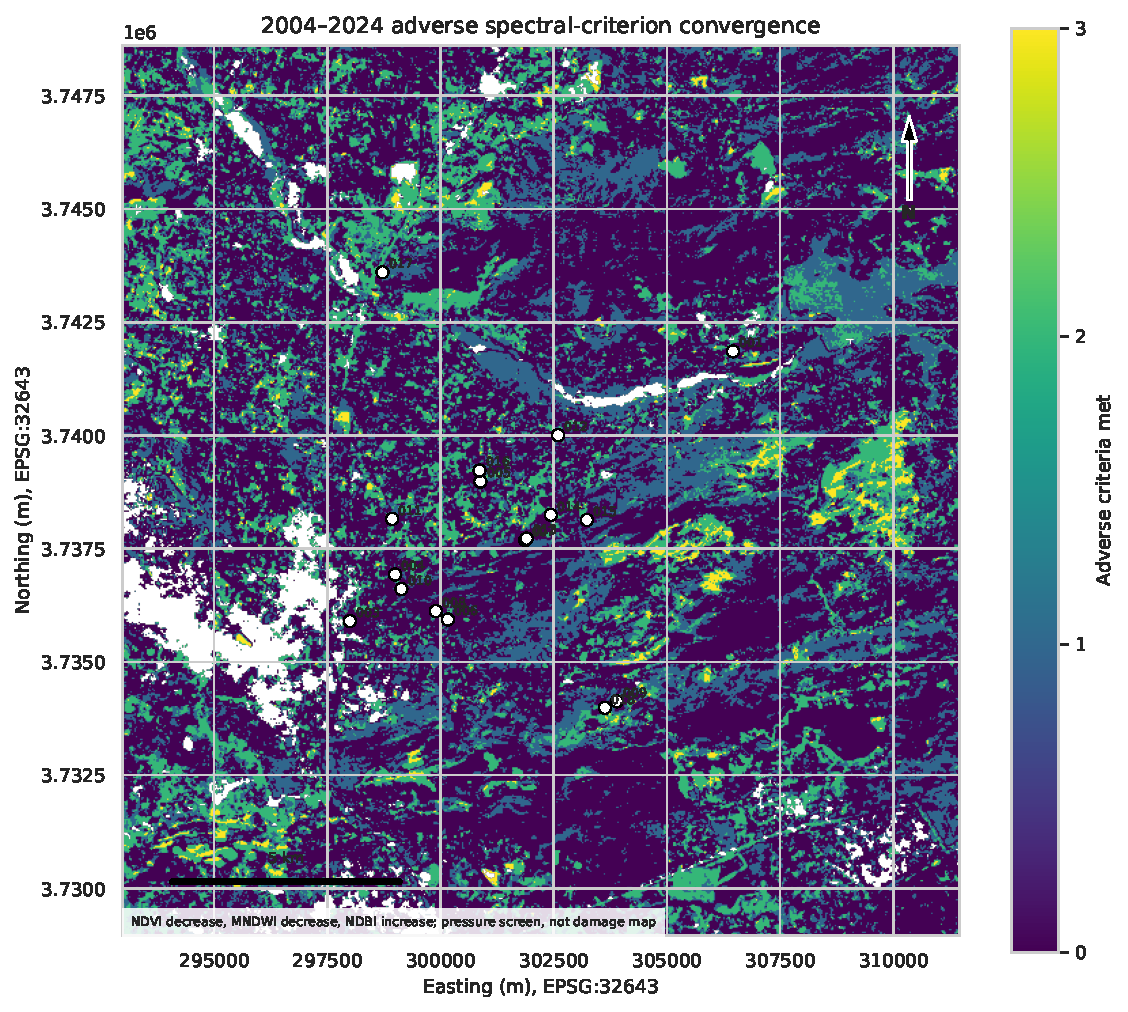
\includegraphics[width=.86\textwidth]{figure_04_spectral_pressure_convergence.pdf}
\caption{Convergence of adverse endpoint spectral criteria on the common E2004--E2024 mask. Values count coincident empirical criteria, with a denominator of 386,280 cells. The map is a landscape screen, not an observation of heritage damage.}\label{fig:convergence}
\end{figure}

\subsection{Priority depends on the uncertainty being considered}
Giri complex had the largest fixed 500 m score (0.591). For the separate integrated context score, the archived 50,000-draw weight analysis gave Giri a central 95\% rank interval of 1--9, with a top-three frequency of 0.774. Spatial resampling instead placed Bhallar at median rank 1 and Giri at median rank 2; the respective intervals were 1--5 and 1--3. These summaries answer different questions: the fixed score assumes the declared architecture, weight perturbation varies that architecture, and spatial resampling varies local spectral support while retaining terrain.

Rank concordance was higher between 500 and 1,000 m ($\rho=0.918$) than between 250 and 1,000 m ($\rho=0.711$). Removing whole domains produced substantial changes: landscape-only ranks correlated 0.325 with the full integrated reference, with a maximum movement of 11 positions; terrain-only ranks correlated 0.830, with a maximum movement of seven. Landscape-only scoring placed Sirkap first, whereas terrain-only scoring placed Bhallar first. A single leader therefore conceals materially different inspection rationales (Fig.~\ref{fig:ranks}).

\begin{figure}[tbp]\centering
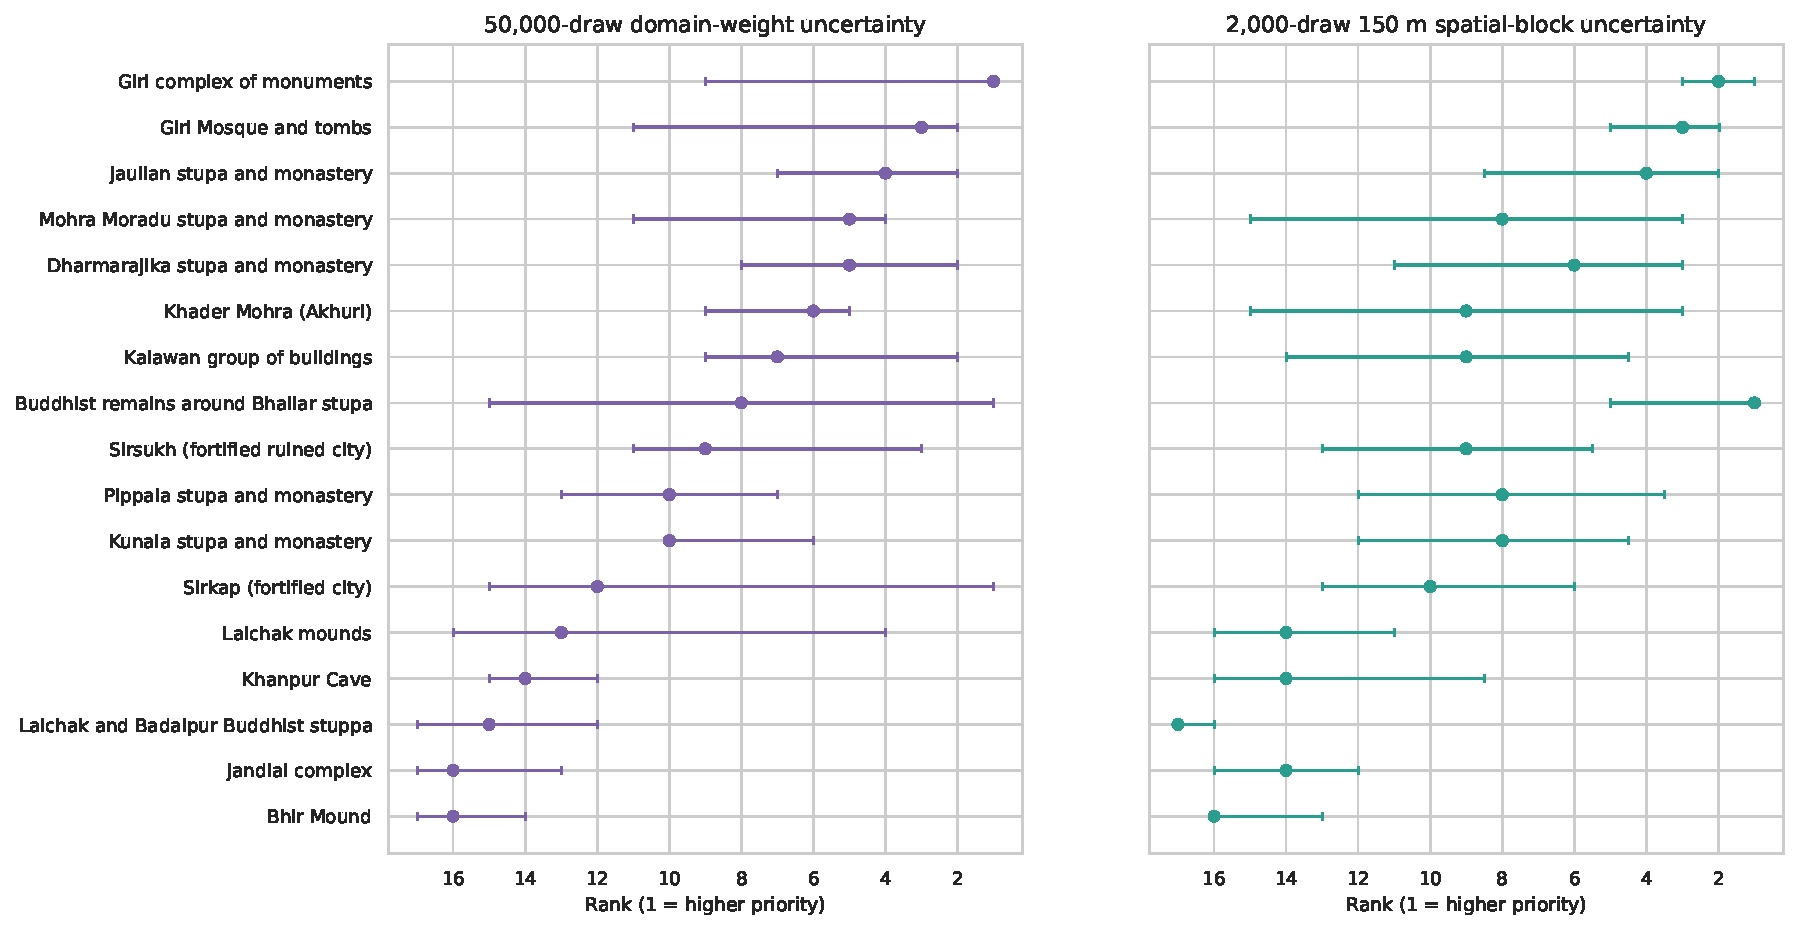
\includegraphics[width=\textwidth]{figure_13_rank_uncertainty.pdf}
\caption{Archived component-rank sensitivity to weight and spatial perturbations. Intervals and top-set frequencies are conditional on their respective resampling designs. They do not combine every measurement, positional or modelling uncertainty. Full component tables and additional joint-uncertainty experiments accompany the notebook.}\label{fig:ranks}
\end{figure}

\subsection{Climate interpretation is product- and window-dependent}
Open-Meteo annual precipitation decreased by 10.30 mm year$^{-1}$ and annual mean temperature increased by 0.0418~$^\circ$C year$^{-1}$. The corrected residual-block intervals and annual-family adjusted probabilities are reported in Supplementary Table~S2. The point slopes were reproducible; their interpretation remained conditional on the selected gridded product.

NASA POWER gave opposing point slopes: +29.21 mm year$^{-1}$ for precipitation and $-0.0372$~$^\circ$C year$^{-1}$ for temperature. Annual precipitation agreement was weak across 35 years (Spearman $\rho=0.083$; RMSE 646.74 mm year$^{-1}$). High daily temperature rank agreement coexisted with a mean offset. These discrepancies reveal product sensitivity, without identifying either series as more accurate (Fig.~\ref{fig:weather}).

Acquisition matching also changed the epoch interpretation. E2024 mean antecedent precipitation was 42.47, 221.19 and 852.92 mm over 30, 90 and 365 days, respectively. It was not the wettest epoch under any of these windows: the maxima belonged to E2004, E2019 and E2014, respectively. A calendar-year or product-specific extreme therefore could not be assigned automatically to the satellite composite.

\begin{figure}[tbp]\centering
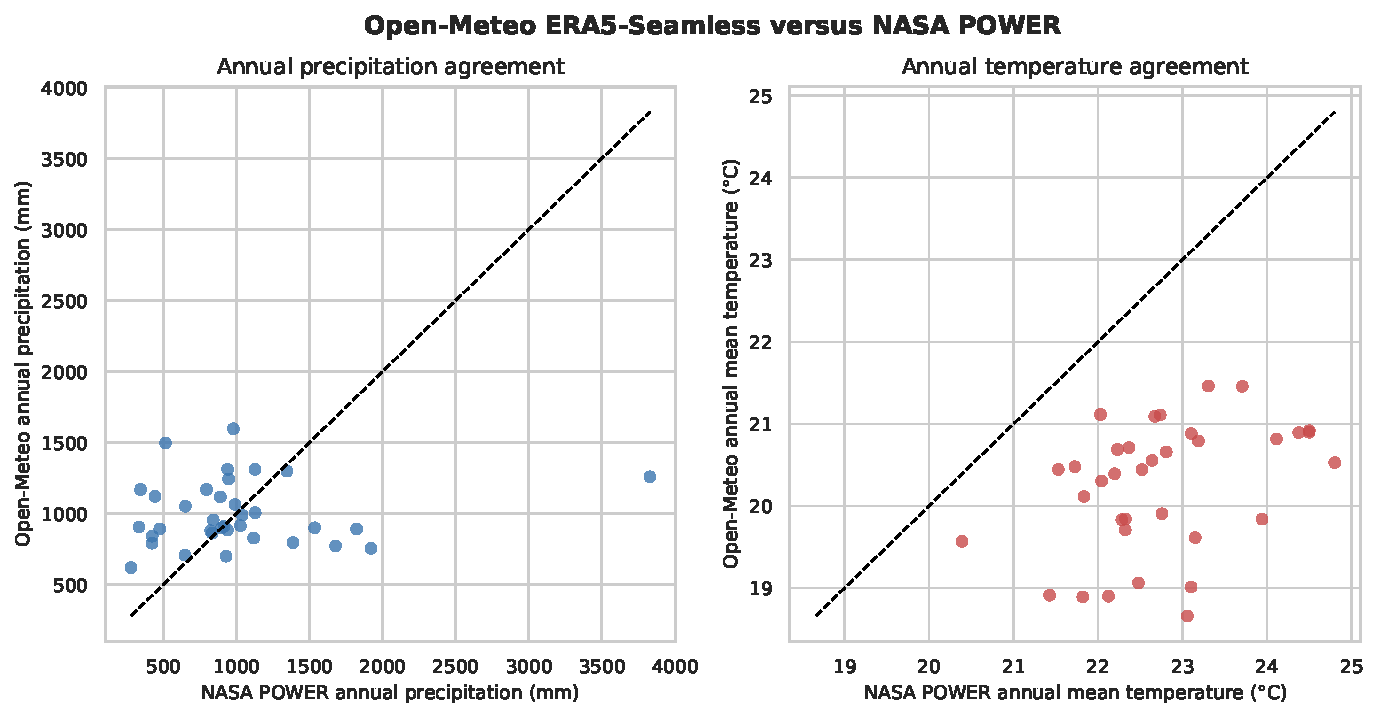
\includegraphics[width=\textwidth]{figure_07_weather_product_comparison.pdf}
\caption{Agreement between the two gridded weather products at matched temporal supports. Differences quantify product dependence, not error relative to station observations. Temporal correlation and absolute agreement are distinct.}\label{fig:weather}
\end{figure}

\subsection{Buffered model selection and diagnostics}
The stricter inner spatial comparison selected \ExtensionModel{} with mean development macro-F1 \ExtensionCV{}. Its outer macro-F1 was \ExtensionFOne{} (95\% test-block interval \ExtensionLow{}--\ExtensionHigh{}), and overall agreement was \ExtensionAgreement{}. Table~\ref{tab:models} reports all seven families, including those that did not lead either comparison. Paired differences, calibration and controls are provided in the Supplementary Information; the outer score was not used to replace the development-selected family.

\begin{table}[tbp]\centering\small
\caption{Seven-family spatial comparison. The primary model is selected using buffered development folds; outer intervals use 2,000 shared test-block resamples.}\label{tab:models}
\begin{tabular}{p{.35\linewidth}rrrr}\toprule
Model & Inner F1 & Outer F1 & 95\% interval & ECE \\\midrule
Random forest (primary) & 0.695 & 0.821 & 0.691--0.835 & 0.014 \\
Logistic regression & 0.655 & 0.807 & 0.680--0.822 & 0.050 \\
MLP & 0.624 & 0.849 & 0.723--0.888 & 0.020 \\
Extra trees & 0.617 & 0.826 & 0.694--0.840 & 0.029 \\
XGBoost & 0.616 & 0.827 & 0.699--0.845 & 0.017 \\
CatBoost & 0.614 & 0.792 & 0.680--0.825 & 0.017 \\
Histogram boosting & 0.611 & 0.846 & 0.704--0.857 & 0.051 \\
\bottomrule\end{tabular}
\end{table}


\ExtensionInterpretation{}

The selected random forest produced the same macro-F1 to numerical precision in Colab and Windows. XGBoost differed by 0.00061 between platforms (0.82687 versus 0.82748); this difference did not alter primary selection. The complete cross-platform comparison is archived.

The historical five-family reproduction yielded macro-F1 \LegacyFOne{}, agreement \LegacyAgreement{} and calibration error \LegacyECE{} for its development-selected MLP. These differ from the original stored targets of 0.830795, 0.833095 and 0.014280. The differences are preserved as historical reproduction discrepancies; targets were not reset to make a rerun pass. The stricter extension uses a different inner protocol and is reported as a separate experiment rather than a replacement claim of exact reproduction.

\section{Discussion}
\subsection{A defensible inspection sequence is conditional}
The main conservation result is the dependence of the inspection order on what the assessment measures. Giri led the fixed composite, Bhallar led the terrain-only ordering, and Sirkap led the landscape-only ordering. These are not interchangeable definitions of priority. A field visit motivated by terrain convergence would examine drainage pathways and local obstructions; one motivated by spectral pressure would examine the origin of surrounding vegetation or surface-cover change. CHIP makes that distinction visible before a map is converted into a management decision.

The broad rank intervals support inspection tiers more strongly than a strict sequence from first to seventeenth. A component that repeatedly enters the early tier warrants attention, while unstable mid-ranked components should be distinguished by the mechanism being investigated and practical survey constraints. The simulation frequencies do not prescribe budgets: access, cultural significance, urgency and specialist judgement were not encoded in the score. Those considerations should be documented when an operational inspection programme is developed.

This contribution complements earlier Taxila work that included ground observations \citep{khan2022taxila}. It does not supersede that evidence or infer an improvement in damage detection. More generally, multi-hazard overlays become easier to assess when their decision sensitivity is exposed alongside the map \citep{guerriero2022derwent,romao2022risk}. The transferable element is the procedure for tracing an inspection recommendation through sources, transformations and uncertainty assumptions; the Taxila weights and empirical thresholds should not be exported unchanged to another property.

\subsection{Stronger models cannot repair an indirect target}
The buffered extension broadens the computational comparison and removes hidden random early-stopping validation. Its difficult inner folds show why geographic label support matters: water was sufficiently concentrated that one training fold contained none. Retaining that limitation is more informative than relaxing the split until every model performs well. Paired test-block intervals also prevent small point-score differences from being presented automatically as improvements.

Nevertheless, the task remains reproduction of a weak label product. Labels are temporally offset from the satellite features and were sampled with class quotas. Overall agreement is therefore conditional on this sample design, not a design-based estimate of landscape accuracy. The reused outer stripe also prevents a confirmatory claim. Recent tabular foundation models demonstrate strong performance on small-data benchmarks \citep{hollmann2025tabpfn}, but their availability does not establish a state-of-the-art heritage-condition result here. Such a claim would require an appropriate independent benchmark, comparable inputs and a target measuring conservation condition.

The next decisive validation should collect independently assessed field observations using a documented component-level protocol. Observers should record material condition and plausible mechanisms separately from landscape context, with agreement between assessors quantified. Evaluation should include components and time periods that were not used to choose the score, thresholds or model. This would test whether the inspection strategy finds actionable conservation problems, rather than merely whether a classifier agrees with another map.

\subsection{Climate context and reproducibility limits}
The opposing weather-product trends prevent a simple claim that regional drying caused the spectral patterns. Acquisition-window matching provides a narrower, defensible interpretation: it describes the meteorological context of the actual observations. Local station data, soil and moisture measurements and higher-frequency satellite observations would be needed to distinguish climatic response from management, seasonality and land-use effects \citep{sesana2021climate,daly2022adaptation}. Four native weather cells cannot resolve component microclimates.

The bootstrap defect illustrates why stored-reference agreement and computational validity must be tested separately. A table can match an archived value while another cell calculates an invalid quantity. The corrected routine preserves the fitted trend for interval estimation and constructs a separate null distribution. Its annual-family probabilities are explicitly separated from older annual/seasonal results. Likewise, unresolved proxy locks remain discrepancies rather than being redefined after execution. These practices make the record auditable without implying that reproducibility alone establishes conservation validity.

Other limitations remain consequential. Point-centred circles are approximations to landscape context, not monument or property footprints. Saraikala's exclusion leaves one inventory component unassessed. Three-year medians and five epochs cannot resolve the timing of short disturbances. Indicator direction, percentile normalisation, DEM routing and structural weights remain assumptions. Spatial resampling does not eliminate sensor error or uncertain labels, and a single study landscape cannot establish external transfer. The framework should therefore guide targeted observation and comparison, with revision as independent evidence becomes available.

\section{Conclusions}\label{sec:conclusions}

The central conservation problem addressed in this study was how to direct limited field-inspection capacity across a distributed archaeological property when relevant evidence differs in spatial support, temporal resolution and meaning. The Climate-linked Heritage Inspection Prioritisation (CHIP) framework responded to this problem by combining five Landsat epochs, regional climate records, terrain and drainage context, and explicit sensitivity analysis in a traceable relative-priority architecture. Its purpose is not to replace condition assessment. It identifies where field teams may obtain the greatest immediate value from inspection, while preserving the distinction between satellite-observed landscape pressure, environmental susceptibility and verified condition of archaeological fabric. The framework consequently offers a disciplined way to move from heterogeneous screening evidence to an inspection sequence without presenting analytical neighbourhoods as legal boundaries or relative scores as absolute measures of deterioration.

The evidence demonstrates both the reach and the selectivity of the screening results. Common endpoint support covered 386,280 cells, or 95.7371\% of the analytical grid. Within that support, 65,391 cells (16.9284\%) met at least two adverse spectral criteria, whereas 5,493 cells (1.4220\%) met all three. These proportions show that spectral convergence was spatially concentrated rather than ubiquitous. The Open-Meteo record indicated an annual precipitation trend of $-10.3037$ mm year$^{-1}$ and an annual mean-temperature trend of $+0.041753$ degrees C year$^{-1}$ over 1991 to 2025, but the opposing NASA POWER trend directions and weak annual precipitation agreement prevented a product-independent climatic conclusion. Scene-matched antecedent windows also showed that E2024 was not uniformly the wettest Landsat epoch. Climate therefore supplies a necessary regional and temporal context for inspection planning, but not reliable component-scale differentiation or a basis for attributing spectral change to a particular forcing.

At the primary 500 m analytical support, the declared equal-domain score placed the Giri complex first with a relative priority score of 0.591176. That result is useful only when reported with its uncertainty. Agreement between the 500 and 1,000 m rankings was high (Spearman $\rho=0.918455$), while agreement between 250 and 1,000 m was lower ($\rho=0.710784$). Across 50,000 domain-weight simulations, Giri retained median rank 1 but ranged from rank 1 to 9 across the central 95\% interval. Across 2,000 spatial-block resamples, Bhallar had median rank 1 with an interval from 1 to 5, whereas Giri had median rank 2 with an interval from 1 to 3. These overlapping distributions change the practical interpretation from a single winner to an initial high-priority group. Factor ablation reinforces that caution: removing MNDWI produced no overlap with the full top five and moved one component by 13 places, while the strong NDVI-pressure and NDBI-pressure correlation ($\rho=0.971707$) exposed residual redundancy. Inspection programmes should therefore consider priority tiers, domain-specific inspection checklists and results across more than one spatial support, rather than allocating resources from a fixed rank alone.

The geographically separated proxy experiment provides a further methodological check, not condition validation. With no development-test block overlap and a 2.01 km exclusion buffer, the development-selected multilayer perceptron reproduced WorldCover-derived proxy labels with macro-F1 0.830795 and balanced accuracy 0.810261 on 4,188 held-out samples. These results show transferable land-cover information in the spectral features, but they do not establish accuracy for archaeological condition or validate the CHIP score. The immediate contribution of the study is therefore a reproducible, uncertainty-aware basis for sequencing field inspection at Taxila, with particular attention to components that remain prominent across fixed, scale-sensitive and resampled summaries. The next decisive step is a stratified field campaign that records fabric condition separately from surrounding land cover, tests drainage, moisture, erosion and encroachment interpretations, resolves Saraikala's geometry, incorporates official component polygons, and validates climate and hydrological context with local observations. Until that evidence is available, CHIP should be used as an adaptive inspection-planning framework whose priorities are revised as field observations accumulate.

\section*{CRediT authorship contribution statement}
\textbf{Mohsin Khan}: Conceptualization, Methodology, Software, Formal analysis,
Data curation, Visualization, Writing -- original draft, Writing -- review \&
editing. \textbf{Sadiq Ullah}: [[roles -- author confirmation required]].
\textbf{Faridoon Khan}: [[roles -- author confirmation required]].
All authors read and approved the submitted manuscript.

\section*{Funding}
[[This research did not receive any specific grant from funding agencies in the
public, commercial, or not-for-profit sectors.]]
% Replace with funder name and grant number if applicable. This statement is
% mandatory at submission and cannot be omitted.

\section*{Declaration of competing interest}
The authors declare that they have no known competing financial interests or
personal relationships that could have appeared to influence the work reported in
this paper.

\section*{Permissions, site access and ethics}
The study used only openly licensed satellite, elevation and reanalysis products
together with the published UNESCO component inventory. No fieldwork, sampling,
excavation or physical intervention at the property was undertaken, and no permit
was therefore required. The analytical neighbourhoods are sampling supports
defined for this study; they are not official property polygons and carry no
statutory or UNESCO buffer-zone status. Component coordinates are published
inventory points reported at their published precision.
[[Confirm whether the Department of Archaeology and Museums and/or the Punjab
Archaeology Department should be acknowledged for inventory access.]]

\section*{Acknowledgements}
The authors thank the USGS/NASA Landsat programme, ESA WorldCover, Open-Meteo,
the NASA POWER project, OpenStreetMap contributors, Natural Earth and
geoBoundaries for open access to the products used here.
[[Add individual and institutional acknowledgements.]]

\section*{Data and code availability}
All derived data, analysis code, configurations, spatial split records,
per-sample model probabilities and result checksums required to reproduce every
number, figure and table in this article are archived at
[[permanent DOI -- deposit required before submission, e.g. Zenodo]].
The archive carries a SHA-256 manifest covering 157 evidence files and includes
the deterministic decision-analysis scripts used for the reconstructed design.
Code is released under [[code licence]] and derived data under
[[data licence]]. Original third-party satellite, land-cover and reanalysis
payloads remain subject to their providers' terms and are re-acquirable with the
documented acquisition scripts and request manifests supplied in the archive.
Identifying repository details are withheld from the anonymised manuscript and
supplied separately to the editor. The workflow begins from documented derived
data; source manifests describe upstream acquisition and preprocessing.

\section*{Declaration of generative AI and AI-assisted technologies}
During preparation of this work, the authors used AI-assisted tools (OpenAI
ChatGPT/Codex and Anthropic Claude) to assist with code development and review,
experiment execution, independent reproducibility and statistical auditing,
schematic preparation, and manuscript drafting and editing. The authors are
responsible for reviewing the code, numerical results, references and
interpretations and for approving the final submission. No tool was treated as an
author or as scientific evidence.

\bibliographystyle{unsrtnat}
\bibliography{references}
\end{document}
